\newpage
\begin{center}
  \huge{Codierungstheorie}
\end{center}

\section{Grundbegriffe und einfache Beispiele}
  \subsection{Codierung (Kanalcodierung)}
    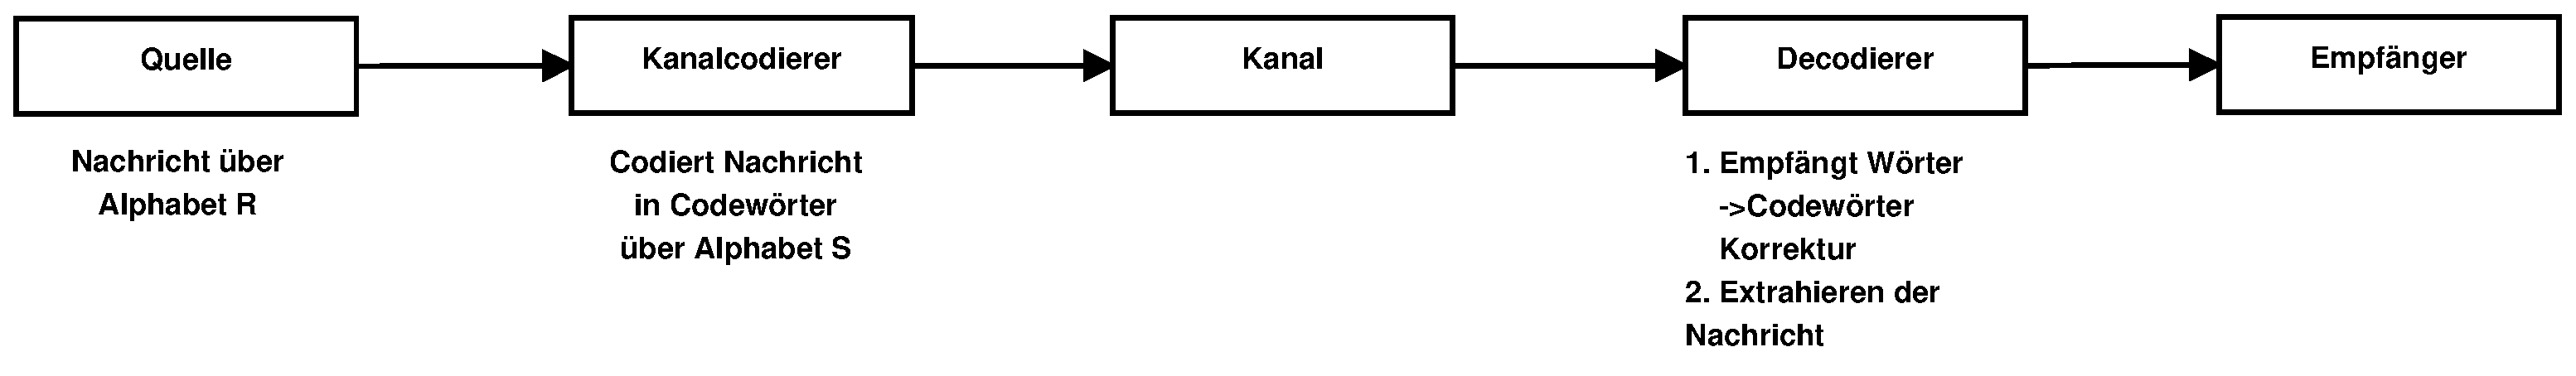
\includegraphics[width=\textwidth]{eps/pic02.eps}
    Ziele:
    \begin{itemize}
      \item Sicherung von Daten bei der Übertragung / Speicherung gegen
      Störungen, Fehler, etc.
      \item Möglichst viele Fehler erkennen und gegebenfalls korrigieren.
      \item Aufwand für Codierung und Decodierung soll nicht zu hoch sein.
    \end{itemize}
    Grundprinzip: Hinzufügen systematischer Redundanz.\\
    Fehlererkennung: Geringe Redundanz
    Fehlerkorrektur: Größere Redundanz, größerer Aufwand
  \subsection{Beispiele}
    \begin{enumerate}[a)]
      \item Parity- Check- Code
        $R=\lrc{0,1}$\\
        Nachricht wird in Blöcke von Länge $k$ zerlegt. Füge an jeden Block Bit
        an, so dass die Anzahl der Einsen im Block der Länge $k+1$ gerade ist
        (also 1 für ungerade, 0 für gerade).\\
        $k=2$:\\
        $00\rightarrow000\\
        01\rightarrow011\\
        10\rightarrow101\\
        11\rightarrow110$\\
        1 Fehler wird erkannt (kann nicht korrigiert werden). 2 Fehler können
        nicht erkannt werden.
      \item Wiederholungscode: Nachricht zerlegt in Blöcke der Länge $k$. Jeder
        Block wird $m$ mal gesendet. $k=2$, $m=3$\\
        $01\rightarrow000000\\
        01\rightarrow010101\\
        10\rightarrow101010\\
        11\rightarrow111111$\\
        1 Fehler lässt sich korrigieren.
      \item Codiere Blöcke der Länge 2 wiefolgt:\\
        $00\rightarrow00000\\
        01\rightarrow01101\\
        10\rightarrow10110\\
        11\rightarrow11011$\\
        1- Fehler- korrigierend:\\
        Decodierung: Such das \gqm{nächste} Codeword zum empfangenen Wort. Je
        zwei Codewörter unterscheiden sich an mindestens 3 Stellen.\\
        2- Fehler- erkennend: Kann jedoch nicht korrigiert werden, da Abstand
        zu zwei gültigen Worten 2 ist.
    \end{enumerate}
  \subsection{GTIN- Prüfzifferncode (GTIN-13)}
    \begin{enumerate}[a)]
      \item GTIN=Global Trade Item Number (früher EAN-13)\\
        12- stelliger Code, $R=S=\lrc{0,...,9}$. Erste 12 Ziffern ensprechen
        Information, 13. Ziffer ist die Prüfziffer\\
        $c_1...c_{13}:c_1...c_{12}$\\
        Herstellungsland (in der Regel die ersten drei Ziffern, Deutschland:
        400-440)\\
        Hersteller (in der Regel $c_4,...,c_8$ (4-6 Ziffern)\\
        Produkt (in der Regel $c_9,...,c_{12}$ (3-5 Ziffern)\\
        $c_{13}$ wird so gewählt, dass gilt:
        $c_1+3c_2+c_3+3c_4+...+c_{11}+3c_{12}+c_{13}\equiv 0(\mod 10)$\\
        $c_{13}=(-c_1+3c_2-c_3-...-3c_12)\mod 10$\\
        Änderung einer Ziffer wird erkannt. $x\mapsto 3x\mod 10$ ist bijektiv
        ($\ggT(3,10)=1$)
      \item Übersetzung der GTIN- 13 in Barcode:\\
        Exkurs, spar ich mir.
    \end{enumerate}

\section{Blockcodes}
	\subsection{Definition}
		$S$ endliche Menge (Alphabet), $n\in\mn$\\
		\textbf{Blockcode} $\mathcal{C}$ der \textbf{(Block-)Länge} $n$ über $S$ ist Teilmenge von $S^n=S\underbrace{\times\dots\times}_{n}S$.\\
		Elemente von $\mathcal{C}$: \textbf{Codewörter}\\
		$S=\lrc{0,1}$: \textbf{binärer Blockcode}\\
		Klar ist $\lrabs{\mathcal{C}}\leq\lrabs{S^n}=\lrabs{S}^n$\\
		Ist $\lrabs{\mathcal{C}}=m$, so lassen sich $m$ Informationssymbole (oder Blöcke) durch je ein Codewort coieren.
	
	\subsection{Definition}
		$S$ endliches Alphabet, $n\in\mn$\\
		$a=\lrr{S_1,\dots,S_n}, b=\lrr{t_1,\dots,t_n}\in S^n$\\
		$d\lrr{a,b}=\lrabs{\lrc{i:1\leq i\leq n, s_i\neq t_i}}$ \textbf{Hamming-Abstand} von $a$ und $b$\\
		(R.W. Hamming, 1915-1998; C. Shannon)
		
	\subsection{Bemerkung}
		\subExBegin{a)}
			\item $a,b,c\in S^n \Rightarrow d\lrr{a,c}\leq d\lrr{a,b}+d\lrr{b,c}$ (Dreiecksungleichung)
			
				$a=\lrr{a_1,\dots,a_n}, b=\lrr{b_1,\dots,b_n}, c=\lrr{c_1,\dots,c_n}$\\
				$\Rightarrow a_i\neq c_i\Rightarrow a_i\neq b_i$ oder $c_i\neq b_i$
			\item Ist $S$ abelsche Gruppe (bzgl. $+$), so gilt\\
				$\forall a,b,c\in S^n: d\lrr{a,b}=d\lrr{a+c,b+c}$\\
				$\lrr{a_1,\dots,a_n}+\lrr{c_1,\dots,c_n}:=\lrr{a_1+c_1,\dots, a_n+c_n}$
			\item Wird $x\in\mathcal{C}$ gesendet und $y\in S^n$ empfangen und $d\lrr{x,y}=k$, so sind $k$ Fehler aufgetreten.
		\subExEnd
		
	\subsection{Definition}
		\subExBegin{a)}
			\item \textbf{Hamming-Decodierung} für Blockcode $\mathcal{C}\mpo S^n$
			
				Wird $y\in S^n$ empfangen, so wird $y$ als ein $x'\in\mathcal{C}$ decodiert mit $d\lrr{x',y}=\min\lrc{d\lrr{x,y}:x\in\mathcal{C}}$ (nicht notwendig eindeutig!)\\
				Hamming-Decodierung ist bestmöglich, wenn alle Codewörter mit der gleichen Wahrscheinlichkeit $p<\frac{1}{2}$ gestört werden und wenn jedes Codewort gleich wahrscheinlich ist.
			\item $\mathcal{C}$ Blockcode in $S^n$, $\lrabs{\mathcal{C}}>1$\\
				\textbf{Minimalabstand} $d\lrr{\mathcal{C}}$ von $\mathcal{C}$: $d\lrr{\mathcal{C}}=\min\lrc{d\lrr{x,y}:x,y\in\mathcal{C} x\neq y}$
			\item Blockcode $\mathcal{C}$ heißt \textbf{t-Fehler-korrigierend}, falls $d\lrr{\mathcal{C}}\geq 2t+1$, $\mathcal{C}$ heißt \textbf{t-Fehler-erkennend}, falls $d\lrr{\mathcal{C}}\geq t+1$
		\subExEnd
		
	\subsection{Bemerkung}
		\subExBegin{a)}
			\item Ist $d\lrr{\mathcal{C}}\geq 2t+1$, so sind die \gqm{Kugeln} vom Radius $t$ um Codewörter $x\in\mathcal{C}$, $K_t\lrr{x}=\lrc{y\in S^n: d\lrr{x,y}\leq t}$, sind disjunkt.
			
				Angenommen $x\in\mathcal{C}$ wird gesendet, $y\in S^n$ wird empfangen, maximal $t$ Fehler seien aufgetreten. $d\lrr{x,y}\leq t$ Bei Hamming-Decodierung wird dann $y$ wieder zu $x$ decodiert, denn jedes andere $x'\in\mathcal{C}$ hat Abstand $>t$ von $y$.
				
			\item Ist $d\lrr{\mathcal{C}}\geq t+1$, $x\in\mathcal{C}$ wird gesendet, $y\in S^n$ empfangen, max. $t$ Fehler seien aufgetreten.\\
				$d\lrr{x,y}\leq t$. Also ist $y\notin\mathcal{C}$ (falls mindestens ein Fehler aufgtreten ist.
		\subExEnd
		
	\subsection{Beispiele}
		\subExBegin{a)}
			\item Parity-Check-Code\\
				$\mathcal{C}=\lrc{\lrr{c_1,\dots,c_n}:c_i\in\mz^2,\sum c_i\equiv 0\lrr{\mbox{mod }2}}$\\
				$d\lrr{\mathcal{C}}=2$\\
				$\lrr{c_1,\dots,c_{n-2},c_{n-1},c_n}\in\mathcal{C}$\\
				$\lrr{c_1,\dots,c_{n-2},\overline{c_{n-1}},\overline{c_n}}\in\mathcal{C}$\\
				$\Rightarrow\mathcal{C}$ ist $1$-Fehler-erkennend.
			\item $m$-facher-Wiederholungscode: $d\lrr{\mathcal{C}}=m$\\
				$\mathcal{C}=\lrc{\lrr{0,\dots,0},\lrr{1,\dots,1},\lrr{2,\dots,2},\dots}$\\
				$\mathcal{C}$ ist $\floor{\frac{m-1}{2}}$-Fehler-korrigierend.\\
				$d\lrr{\mathcal{C}}\geq 2t+1$ Für alle $x,x'\in \mathcal{C}, x\neq x': K_t\lrr{x}\mand K_t\lrr{x'}=\mvoid$
		\subExEnd
		
	\subsection{Definition}
		Sei $\mathcal{C}$ Blockcode über $S$ der Länge $n$.\\
		$\mathcal{C}$ heißt \textbf{perfekt}, falls es $t\in\mn_0$ gibt mit $S^n=\ouset{\mor}{\bullet}{x\in\mathcal{C}}K_t\lrr{x}$ (disjunkte Vereinigung)